% =====================================================================
%  IT5208 – Thống kê ứng dụng (HUST) – Báo cáo: Quá trình Bernoulli
%  Biên dịch: xelatex report.tex  (chạy 2 lần để có mục lục và tham chiếu)
%  Cấu trúc thư mục cần có:
%     report.tex
%     figures/  sample_paths.png, binomial.png, geometric.png, poisson_limit.png
%     code/     bernoulli_process.py, demo.py
% =====================================================================
\documentclass[12pt,a4paper]{article}

% ---------- Ngôn ngữ và phông chữ ----------
\usepackage{fontspec}
\usepackage{babel}
\babelprovide[import,main]{vietnamese}
\IfFontExistsTF{Times New Roman}{\setmainfont{Times New Roman}}{\setmainfont{Liberation Serif}}
\IfFontExistsTF{Consolas}{\setmonofont[Scale=0.9]{Consolas}}{\setmonofont[Scale=0.9]{Liberation Mono}}

% ---------- Gói chung ----------
\usepackage[margin=2.5cm]{geometry}
\usepackage{amsmath,amssymb,amsthm}
\usepackage{graphicx}
\usepackage{booktabs,tabularx,array,multirow}
\usepackage{caption}
\usepackage{placeins}
\usepackage{enumitem}
\usepackage{xcolor}
\usepackage{listings}
\usepackage{tikz}
\usepackage{pgfplots}
\pgfplotsset{compat=1.17}
\usetikzlibrary{arrows.meta,positioning,calc,decorations.pathreplacing,automata}
\usepackage[hidelinks]{hyperref}

\graphicspath{{figures/}{../figures/}}

% ---------- Bảng màu theo template HUST ----------
\definecolor{hustred}{HTML}{BF1F33}
\definecolor{hustgold}{HTML}{E49B09}
\definecolor{hustgray}{HTML}{595959}
\definecolor{hustlight}{HTML}{F2F2F2}
\definecolor{husttint}{HTML}{FBECEE}

\captionsetup{font=small,labelfont={bf,color=hustred}}
\setlist{itemsep=2pt,topsep=4pt}

\lstset{
  language=Python, basicstyle=\ttfamily\small, keywordstyle=\color{hustred}\bfseries,
  commentstyle=\color{hustgray}\itshape, stringstyle=\color{hustgold!80!black},
  numbers=left, numberstyle=\tiny\color{hustgray}, frame=single, rulecolor=\color{hustgray!40},
  backgroundcolor=\color{hustlight}, breaklines=true, columns=fullflexible, showstringspaces=false,
  captionpos=b
}
\renewcommand{\lstlistingname}{Đoạn mã}

\theoremstyle{definition}
\newtheorem{definition}{Định nghĩa}[section]
\newtheorem{proposition}{Mệnh đề}[section]
\newtheorem{example}{Ví dụ}[section]
\theoremstyle{remark}
\newtheorem*{remark}{Nhận xét}

% ---------- Ký hiệu ----------
\newcommand{\Prob}{\mathbb{P}}
\newcommand{\E}{\mathbb{E}}
\newcommand{\Var}{\operatorname{Var}}
\newcommand{\Bern}{\operatorname{Bernoulli}}
\newcommand{\Bin}{\operatorname{Binomial}}
\newcommand{\Geo}{\operatorname{Geometric}}
\newcommand{\NB}{\operatorname{NegBin}}
\newcommand{\Pois}{\operatorname{Poisson}}

\newcommand{\checkme}[1]{\textcolor{hustred}{\textbf{[CẦN KIỂM TRA: #1]}}}

\title{\textbf{\color{hustred} Quá trình Bernoulli (Bernoulli process)}\\[4pt]
  \large Báo cáo môn IT5208 – Thống kê ứng dụng}
\author{Nhóm: [Tên nhóm]\\ Thành viên: [Thành viên]\\[2pt]
  \small Đại học Bách khoa Hà Nội}
\date{\today}

\begin{document}
\maketitle

\begin{abstract}
Báo cáo trình bày quá trình Bernoulli – quá trình ngẫu nhiên (stochastic process) đơn giản nhất với thời gian
rời rạc và hai trạng thái. Chúng tôi nêu định nghĩa và các đại lượng dẫn xuất (quá trình đếm, thời gian chờ,
khoảng thời gian giữa hai lần thành công), chứng minh các tính chất chính (không nhớ, gia số độc lập và dừng,
tách/ghép, giới hạn Poisson), so sánh với quá trình Poisson, xích Markov, bước ngẫu nhiên và quá trình Wiener,
trình bày ba ứng dụng thực tế, và cuối cùng cài đặt mô phỏng bằng Python chỉ dùng bộ sinh số đều
\texttt{random.random()}. Kết quả mô phỏng khớp với lý thuyết với sai lệch dưới 1\%.
\end{abstract}

\tableofcontents
\newpage

% =====================================================================
\section{Giới thiệu}\label{sec:intro}
Nhiều hiện tượng thực tế chỉ có hai kết cục và lặp lại theo từng bước: một sản phẩm trên dây chuyền lỗi hay
không, một gói tin truyền thành công hay bị mất, một người dùng có chuyển đổi (mua hàng, đăng ký) hay không.
Nếu các bước (gần như) độc lập và xác suất ``thành công'' không đổi, toàn bộ dãy kết cục được mô tả bởi
\emph{quá trình Bernoulli}. Từ mô hình này, hai loại câu hỏi được trả lời một cách thống nhất:
\begin{itemize}
  \item \textbf{Đếm}: sau $n$ bước có bao nhiêu lần thành công?
  \item \textbf{Chờ}: phải chờ bao lâu đến lần thành công đầu tiên, hay lần thứ $r$?
\end{itemize}
Báo cáo gồm bốn phần theo yêu cầu đề bài: định nghĩa và tính chất (Mục~\ref{sec:def}), so sánh với các quá
trình ngẫu nhiên khác (Mục~\ref{sec:compare}), ứng dụng thực tế (Mục~\ref{sec:app}), cài đặt Python và kết quả
mô phỏng (Mục~\ref{sec:code} và~\ref{sec:results}). Phần lý thuyết chủ yếu dựa theo~\cite{bertsekas}, có
tham khảo thêm~\cite{ross,grimmett}.

\paragraph{Ký hiệu.} Xuyên suốt báo cáo: $p$ là xác suất thành công, $q = 1-p$; $X_k$ là kết cục ở bước $k$;
$S_n$ là số lần thành công sau $n$ bước; $T_r$ là thời điểm thành công thứ $r$; $L_k = T_k - T_{k-1}$ là
khoảng thời gian giữa hai lần thành công liên tiếp.

% =====================================================================
\section{Định nghĩa và các tính chất}\label{sec:def}

\subsection{Định nghĩa}
\begin{definition}[Quá trình Bernoulli]\label{def:bern}
Cho $p\in[0,1]$. \emph{Quá trình Bernoulli} với tham số $p$ là dãy biến ngẫu nhiên $X_1, X_2, \dots$
\textbf{độc lập, cùng phân phối} (i.i.d.) với
\begin{equation}\label{eq:bern}
  \Prob(X_k = 1) = p, \qquad \Prob(X_k = 0) = 1-p = q, \qquad k = 1,2,\dots
\end{equation}
Biến cố $\{X_k = 1\}$ gọi là \emph{thành công} (hay ``đến'', arrival) tại thời điểm $k$.
\end{definition}

Đây là quá trình với \textbf{thời gian rời rạc} $k\in\{1,2,\dots\}$ và \textbf{không gian trạng thái rời rạc}
$\{0,1\}$; toàn bộ phân phối của quá trình được xác định bởi một tham số duy nhất $p$. Với mỗi $k$,
\begin{equation}\label{eq:bern-moments}
  \E[X_k] = p, \qquad \Var(X_k) = \E[X_k^2] - p^2 = p - p^2 = pq.
\end{equation}
Do tính độc lập, xác suất của một đường mẫu hữu hạn $(x_1,\dots,x_n)\in\{0,1\}^n$ là
\begin{equation}\label{eq:path-prob}
  \Prob(X_1 = x_1, \dots, X_n = x_n) = p^{\,s} q^{\,n-s}, \qquad s = x_1 + \dots + x_n,
\end{equation}
tức là chỉ phụ thuộc vào \emph{số} lần thành công chứ không phụ thuộc vào vị trí của chúng.

Hình~\ref{fig:timeline} minh hoạ 12 bước đầu của đường mẫu dùng trong phần demo ($p = 0{,}3$), với các thời
điểm thành công $T_1=1, T_2=4, T_3=9, T_4=10$ và khoảng cách $L_1=1, L_2=3, L_3=5, L_4=1$.

\begin{figure}[ht]
\centering
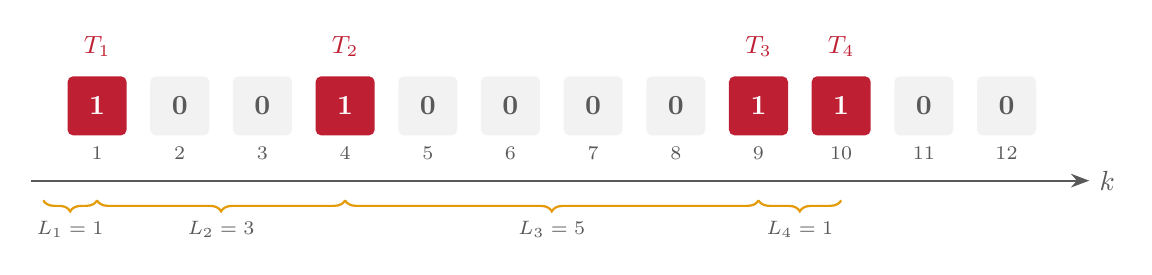
\begin{tikzpicture}[x=1.05cm,y=1cm,
  cell/.style={draw=none,minimum size=0.75cm,rounded corners=2pt,font=\bfseries}]
  \def\bits{1,0,0,1,0,0,0,0,1,1,0,0}
  \foreach \b [count=\i] in \bits {
    \ifnum\b=1
      \node[cell,fill=hustred,text=white] (c\i) at (\i,0) {1};
    \else
      \node[cell,fill=hustlight,text=hustgray] (c\i) at (\i,0) {0};
    \fi
    \node[font=\scriptsize,text=hustgray] at (\i,-0.6) {\i};
  }
  \draw[-{Stealth},hustgray,thick] (0.2,-0.95) -- (13.0,-0.95) node[right] {$k$};
  \foreach \t/\j in {1/1,4/2,9/3,10/4}
    \node[text=hustred,font=\small\bfseries] at (\t,0.75) {$T_{\j}$};
  \foreach \a/\b/\l/\j in {0.35/1/1/1,1/4/3/2,4/9/5/3,9/10/1/4}{
    \draw[decorate,decoration={brace,mirror,amplitude=4pt},hustgold,thick]
      (\a,-1.2) -- (\b,-1.2) node[midway,below=4pt,text=hustgray,font=\scriptsize] {$L_{\j}=\l$};
  }
\end{tikzpicture}
\caption{Một đường mẫu của quá trình Bernoulli ($p=0{,}3$, 12 bước đầu của demo): ô đỏ là thành công,
$T_r$ là thời điểm thành công thứ $r$, $L_k$ là khoảng cách giữa hai lần thành công liên tiếp.}
\label{fig:timeline}
\end{figure}

\subsection{Quá trình đếm và phân phối nhị thức}
\begin{definition}
\emph{Quá trình đếm} (counting process) của quá trình Bernoulli là $S_0 = 0$ và
\begin{equation}\label{eq:Sn}
  S_n = X_1 + X_2 + \dots + X_n, \qquad n \ge 1.
\end{equation}
\end{definition}

\begin{proposition}\label{prop:binomial}
$S_n \sim \Bin(n,p)$, nghĩa là
\begin{equation}\label{eq:binom-pmf}
  \Prob(S_n = k) = \binom{n}{k} p^k q^{n-k}, \qquad k = 0,1,\dots,n,
\end{equation}
và
\begin{equation}\label{eq:binom-moments}
  \E[S_n] = np, \qquad \Var(S_n) = npq.
\end{equation}
\end{proposition}
\begin{proof}
Theo~\eqref{eq:path-prob}, mỗi đường mẫu có đúng $k$ số 1 có xác suất $p^kq^{n-k}$, và có $\binom{n}{k}$ đường
như vậy, suy ra~\eqref{eq:binom-pmf}. Tính tuyến tính của kỳ vọng cho $\E[S_n] = \sum_k \E[X_k] = np$; vì các
$X_k$ độc lập nên phương sai cộng được: $\Var(S_n) = \sum_k \Var(X_k) = npq$.
\end{proof}

Hình~\ref{fig:tree} là cây nhị thức (dạng lưới tái hợp) 3 bước: mỗi nhánh lên ứng với thành công (xác suất
$p$), nhánh xuống ứng với thất bại (xác suất $q$). Số đường đi đến nút $S_3=k$ là $\binom{3}{k}=1,3,3,1$.

\begin{figure}[ht]
\centering
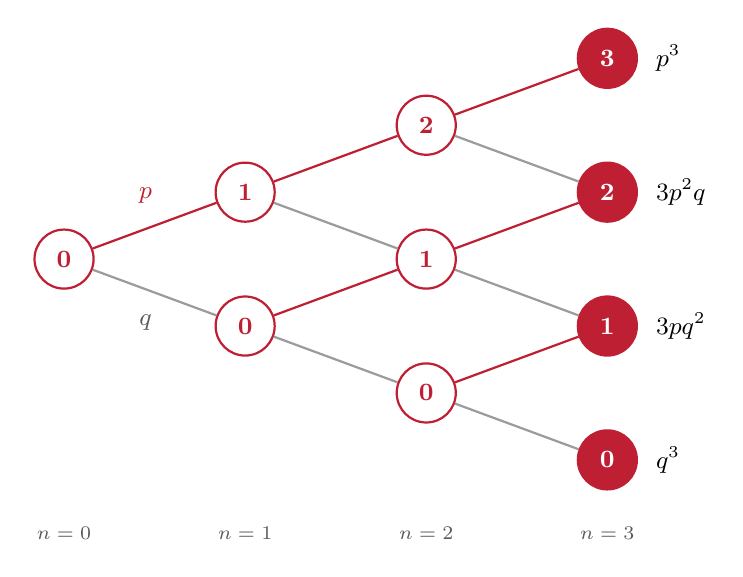
\begin{tikzpicture}[x=2.3cm,y=0.85cm,
  nd/.style={circle,draw=hustred,thick,minimum size=0.75cm,font=\small\bfseries,text=hustred,fill=white},
  leaf/.style={circle,draw=hustred,thick,minimum size=0.75cm,font=\small\bfseries,text=white,fill=hustred}]
  \foreach \n in {0,...,3}{
    \foreach \k in {0,...,\n}{
      \pgfmathsetmacro{\yy}{2*\k-\n}
      \ifnum\n=3
        \node[leaf] (n\n\k) at (\n,\yy) {\k};
      \else
        \node[nd] (n\n\k) at (\n,\yy) {\k};
      \fi
    }
    \node[text=hustgray,font=\scriptsize] at (\n,-4.1) {$n=\n$};
  }
  \foreach \n in {0,1,2}{
    \pgfmathtruncatemacro{\m}{\n+1}
    \foreach \k in {0,...,\n}{
      \pgfmathtruncatemacro{\kk}{\k+1}
      \draw[hustred,thick] (n\n\k) -- (n\m\kk);
      \draw[hustgray!60,thick] (n\n\k) -- (n\m\k);
    }
  }
  \node[text=hustred,font=\small] at (0.45,0.95) {$p$};
  \node[text=hustgray,font=\small] at (0.45,-0.95) {$q$};
  \node[right=3pt of n33,font=\small] {$p^3$};
  \node[right=3pt of n32,font=\small] {$3p^2q$};
  \node[right=3pt of n31,font=\small] {$3pq^2$};
  \node[right=3pt of n30,font=\small] {$q^3$};
\end{tikzpicture}
\caption{Cây nhị thức 3 bước. Nhãn trong nút là $S_n$; xác suất ở mỗi lá là $\Prob(S_3=k)=\binom{3}{k}p^kq^{3-k}$.}
\label{fig:tree}
\end{figure}

\subsection{Thời gian chờ: phân phối hình học và nhị thức âm}
\begin{definition}
Thời điểm thành công thứ $r$ là $T_r = \min\{n \ge 1: S_n = r\}$, $r = 1,2,\dots$ (quy ước $T_0 = 0$).
Khoảng thời gian giữa hai lần thành công là $L_k = T_k - T_{k-1}$.
\end{definition}

\begin{proposition}[Thời gian chờ lần thành công đầu tiên]\label{prop:geo}
$T_1 \sim \Geo(p)$ (với $p>0$):
\begin{equation}\label{eq:geo}
  \Prob(T_1 = k) = q^{k-1}p,\quad k\ge 1;\qquad \Prob(T_1 > k) = q^k;\qquad
  \E[T_1] = \frac1p,\quad \Var(T_1) = \frac{q}{p^2}.
\end{equation}
\end{proposition}
\begin{proof}
$\{T_1 = k\} = \{X_1 = \dots = X_{k-1} = 0, X_k = 1\}$ nên $\Prob(T_1=k)=q^{k-1}p$, và
$\{T_1 > k\} = \{X_1=\dots=X_k=0\}$ nên $\Prob(T_1>k)=q^k$. Với $|q|<1$, đạo hàm chuỗi hình học cho
$\sum_{k\ge1} kq^{k-1} = 1/p^2$ và $\sum_{k\ge1}k(k-1)q^{k-2} = 2/p^3$. Do đó $\E[T_1] = p\cdot 1/p^2 = 1/p$,
$\E[T_1(T_1-1)] = pq\cdot 2/p^3 = 2q/p^2$, và
$\Var(T_1) = 2q/p^2 + 1/p - 1/p^2 = q/p^2$.
\end{proof}

\begin{proposition}[Thời điểm thành công thứ $r$]\label{prop:negbin}
$T_r$ có phân phối nhị thức âm (Negative Binomial) $\NB(r,p)$:
\begin{equation}\label{eq:negbin}
  \Prob(T_r = t) = \binom{t-1}{r-1} p^r q^{t-r}, \quad t = r, r+1, \dots;\qquad
  \E[T_r] = \frac rp,\quad \Var(T_r) = \frac{rq}{p^2}.
\end{equation}
\end{proposition}
\begin{proof}
$\{T_r = t\}$ xảy ra khi và chỉ khi $X_t = 1$ và trong $t-1$ bước đầu có đúng $r-1$ thành công. Hai biến cố
này độc lập, nên $\Prob(T_r=t) = \binom{t-1}{r-1}p^{r-1}q^{t-r}\cdot p$. Kỳ vọng và phương sai suy ra từ
Mệnh đề~\ref{prop:interarrival} bên dưới: $T_r = L_1 + \dots + L_r$ là tổng $r$ biến $\Geo(p)$ độc lập.
\end{proof}

\begin{proposition}[Khoảng thời gian giữa các lần thành công]\label{prop:interarrival}
Các biến $L_1, L_2, \dots$ độc lập, cùng phân phối $\Geo(p)$. Do đó $T_r = \sum_{k=1}^r L_k$.
\end{proposition}
\begin{proof}[Phác thảo chứng minh]
Với $\ell_1,\dots,\ell_r\ge1$ và $t_j = \ell_1+\dots+\ell_j$, biến cố
$\{L_1=\ell_1,\dots,L_r=\ell_r\}$ nghĩa là các bước $t_1,\dots,t_r$ là thành công và mọi bước khác trong
$1,\dots,t_r$ là thất bại. Theo~\eqref{eq:path-prob} xác suất của nó là
$p^r q^{t_r - r} = \prod_{j=1}^r q^{\ell_j-1}p$, tức là tích các xác suất hình học.
\end{proof}

\begin{remark}[Quan hệ đối ngẫu giữa đếm và chờ]
Với mọi $r,n$: $\{T_r \le n\} = \{S_n \ge r\}$. Vì thế
$\Prob(T_r \le n) = \sum_{k=r}^{n}\binom nk p^k q^{n-k}$: mọi câu hỏi về thời gian chờ có thể chuyển thành câu
hỏi về quá trình đếm và ngược lại.
\end{remark}

\subsection{Các tính chất quan trọng}
\paragraph{Tính không nhớ (memoryless).} Với mọi $m,k\ge0$,
\begin{equation}\label{eq:memoryless}
  \Prob(T_1 > m+k \mid T_1 > m) = \frac{q^{m+k}}{q^m} = q^k = \Prob(T_1 > k).
\end{equation}
Phân phối hình học là phân phối rời rạc duy nhất trên $\{1,2,\dots\}$ có tính chất này. Tổng quát hơn, với
mọi thời điểm cố định $n$, dãy $X_{n+1}, X_{n+2},\dots$ lại là một quá trình Bernoulli$(p)$ và độc lập với
$X_1,\dots,X_n$ (``quá trình bắt đầu lại'', fresh start). Điều này còn đúng khi $n$ được thay bằng một thời
điểm dừng như $T_r$; đây chính là lý do các $L_k$ độc lập (Mệnh đề~\ref{prop:interarrival}).

\paragraph{Gia số độc lập và dừng.} Với $n,m \ge 0$:
\begin{equation}\label{eq:increments}
  S_{n+m} - S_n = X_{n+1} + \dots + X_{n+m} \sim \Bin(m,p),
\end{equation}
không phụ thuộc $n$ (gia số dừng) và độc lập với $S_1,\dots,S_n$; số thành công trên các khoảng thời gian rời
nhau là độc lập (gia số độc lập).

\paragraph{Tách (thinning).} Mỗi lần thành công được giữ lại với xác suất $r$, độc lập với mọi thứ khác. Quá
trình các thành công được giữ lại $Y_k$ thoả $\Prob(Y_k=1)=pr$ và các $Y_k$ độc lập, tức là
$\Bern(pr)$; phần bị loại là quá trình $\Bern(p(1-r))$. Lưu ý hai quá trình này \emph{không} độc lập với nhau
(không thể cùng bằng 1 ở một bước).

\paragraph{Ghép (merging).} Cho hai quá trình độc lập $X_k\sim\Bern(p_1)$ và $Y_k\sim\Bern(p_2)$. Quá trình
ghép $Z_k = \max(X_k,Y_k)$ (có ít nhất một thành công ở bước $k$) là quá trình Bernoulli với tham số
\begin{equation}\label{eq:merge}
  \Prob(Z_k = 1) = 1 - (1-p_1)(1-p_2) = p_1 + p_2 - p_1p_2 .
\end{equation}
Khác với quá trình Poisson, khi hai thành công trùng bước, quá trình ghép chỉ ghi nhận một lần.

\subsection{Giới hạn Poisson}
\begin{proposition}\label{prop:poisson}
Cố định $\lambda > 0$ và đặt $p = \lambda/n$. Khi $n\to\infty$, với mỗi $k$ cố định,
\begin{equation}\label{eq:poisson-limit}
  \binom nk\Big(\frac\lambda n\Big)^k\Big(1-\frac\lambda n\Big)^{n-k} \longrightarrow
  e^{-\lambda}\frac{\lambda^k}{k!}.
\end{equation}
\end{proposition}
\begin{proof}
Viết vế trái thành
$\dfrac{\lambda^k}{k!}\cdot\dfrac{n(n-1)\cdots(n-k+1)}{n^k}\cdot\Big(1-\dfrac\lambda n\Big)^{n}\cdot
\Big(1-\dfrac\lambda n\Big)^{-k}$. Thừa số thứ hai và thứ tư tiến về 1, thừa số thứ ba tiến về $e^{-\lambda}$.
\end{proof}
Ý nghĩa: khi số phép thử rất lớn và mỗi phép thử hiếm khi thành công, $\Bin(n,p)\approx\Pois(np)$. Nếu chia
trục thời gian liên tục thành các khe độ dài $\delta$ và đặt $p = \lambda\delta$, khi $\delta\to0$ quá trình
Bernoulli hội tụ về \emph{quá trình Poisson} với cường độ $\lambda$; thời gian chờ hình học hội tụ về phân phối
mũ. Hình~\ref{fig:poisson} (Mục~\ref{sec:results}) minh hoạ sự hội tụ với $\lambda=3$.

% =====================================================================
\section{Khác biệt so với các quá trình ngẫu nhiên khác}\label{sec:compare}

Bảng~\ref{tab:compare} so sánh quá trình Bernoulli với bốn quá trình ngẫu nhiên thường gặp. Trong bảng,
bước ngẫu nhiên (random walk) đơn giản được định nghĩa từ quá trình Bernoulli bởi
\begin{equation}\label{eq:rw}
  Y_n = \sum_{k=1}^n (2X_k - 1), \qquad \E[Y_n] = n(2p-1),\quad \Var(Y_n) = 4npq.
\end{equation}

\begin{table}[ht]
\centering
\caption{So sánh quá trình Bernoulli với các quá trình ngẫu nhiên khác.}
\label{tab:compare}
\small
\renewcommand{\arraystretch}{1.3}
\begin{tabularx}{\textwidth}{>{\bfseries\raggedright}p{2.1cm}
  >{\raggedright}X >{\raggedright}X >{\raggedright}X >{\raggedright}X >{\raggedright\arraybackslash}X}
\toprule
Tiêu chí & Bernoulli & Poisson process & Markov chain & Random walk & Wiener process \\
\midrule
Thời gian & Rời rạc, $k=1,2,\dots$ & Liên tục, $t\ge0$ & Rời rạc (bản cơ bản) & Rời rạc & Liên tục \\
Không gian trạng thái & $\{0,1\}$ & $\{0,1,2,\dots\}$ (số đếm $N(t)$) & Rời rạc, hữu hạn hoặc đếm được
  & $\mathbb Z$ & $\mathbb R$ \\
Tính phụ thuộc & $X_k$ i.i.d. & Gia số độc lập, dừng & $X_{n+1}$ phụ thuộc $X_n$
  & Gia số i.i.d.\ $\pm1$; các $Y_n$ phụ thuộc nhau & Gia số độc lập, phân phối chuẩn \\
Thời gian chờ & $\Geo(p)$ & Mũ $\mathrm{Exp}(\lambda)$ & Thời gian lưu tại $i$: $\Geo(1-P_{ii})$
  & Thời điểm chạm mức – không có dạng đơn giản & Không có ``sự kiện'' rời rạc \\
Không nhớ & Có (rời rạc) & Có (liên tục) & Tính Markov: chỉ phụ thuộc hiện tại & Có tính Markov
  & Có tính Markov \\
Tham số & $p$ & $\lambda$ & Ma trận chuyển $P$, phân phối đầu $\pi_0$ & $p$ (xác suất bước $+1$)
  & $\mu,\sigma^2$ \\
\bottomrule
\end{tabularx}
\end{table}

\paragraph{So với quá trình Poisson.} Cả hai đều ``đếm sự kiện'' và đều có gia số độc lập, dừng cùng tính không
nhớ. Khác biệt cốt lõi là thời gian: Bernoulli rời rạc nên thời gian chờ là hình học, Poisson liên tục nên thời
gian chờ là mũ. Quá trình Bernoulli là phiên bản rời rạc của quá trình Poisson, và quá trình Poisson là giới hạn
của quá trình Bernoulli (Mệnh đề~\ref{prop:poisson}).

\paragraph{So với xích Markov.} Xích Markov cho phép trạng thái kế tiếp phụ thuộc trạng thái hiện tại thông qua
ma trận chuyển $P$. Quá trình Bernoulli là xích Markov hai trạng thái đặc biệt có hai hàng của $P$ giống hệt nhau
(Hình~\ref{fig:markov}): khi đó $\Prob(X_{n+1}=1\mid X_n)=p$ bất kể $X_n$, tức là không còn phụ thuộc.

\begin{figure}[ht]
\centering
\begin{tikzpicture}[->,>={Stealth},node distance=3.2cm,thick,
  st/.style={circle,draw=hustred,fill=husttint,minimum size=1cm,font=\bfseries}]
  \node[st] (a) {0};
  \node[st,right=of a] (b) {1};
  \path (a) edge[bend left=25,hustred] node[above,font=\small,text=black] {$a$} (b)
        (b) edge[bend left=25,hustgray] node[below,font=\small,text=black] {$b$} (a)
        (a) edge[loop left,hustgray] node[left,font=\small,text=black] {$1-a$} (a)
        (b) edge[loop right,hustred] node[right,font=\small,text=black] {$1-b$} (b);
  \node[right=1.6cm of b,align=left,font=\small] {
    $P=\begin{pmatrix}1-a & a\\ b & 1-b\end{pmatrix}$\\[6pt]
    Bernoulli$(p)$ $\iff a = p,\ b = q$:\\[2pt]
    $P=\begin{pmatrix}q & p\\ q & p\end{pmatrix}$ (hai hàng như nhau)};
\end{tikzpicture}
\caption{Xích Markov hai trạng thái. Quá trình Bernoulli là trường hợp riêng khi $a = p$ và $b = q$.}
\label{fig:markov}
\end{figure}

\paragraph{So với bước ngẫu nhiên.} Bước ngẫu nhiên~\eqref{eq:rw} là một \emph{hàm} của quá trình Bernoulli:
các bước $2X_k-1\in\{-1,+1\}$ là i.i.d., nhưng bản thân các giá trị $Y_1, Y_2, \dots$ không độc lập (ví dụ
$Y_{n+1}$ chỉ cách $Y_n$ một đơn vị). Không gian trạng thái là $\mathbb Z$ thay vì $\{0,1\}$.

\paragraph{So với quá trình Wiener / quá trình Gauss.} Quá trình Wiener (chuyển động Brown) có thời gian và
trạng thái liên tục, gia số độc lập có phân phối chuẩn; nó là giới hạn (sau khi chuẩn hoá) của bước ngẫu nhiên,
theo định lý Donsker. Quá trình Gauss tổng quát hơn: mọi phân phối hữu hạn chiều là chuẩn nhiều chiều, được xác
định bởi hàm trung bình và hàm hiệp phương sai.

Hình~\ref{fig:relations} tóm tắt quan hệ giữa quá trình Bernoulli và các phân phối/quá trình dẫn xuất.

\begin{figure}[ht]
\centering
\begin{tikzpicture}[node distance=1.2cm and 1.0cm,
  box/.style={draw=hustred,thick,rounded corners=3pt,minimum width=3.0cm,minimum height=1cm,align=center,
              font=\small,fill=white},
  core/.style={box,fill=hustred,text=white,font=\small\bfseries},
  lab/.style={font=\scriptsize\itshape,text=hustgray},
  ar/.style={-{Stealth},thick,hustred}, ar2/.style={-{Stealth},thick,hustgray}]
  \node[core] (B) {Bernoulli$(p)$\\ $X_k$ i.i.d.};
  \node[box,above left=of B] (Bin) {\textbf{Binomial}$(n,p)$\\ đếm $S_n$};
  \node[box,above right=of B] (Geo) {\textbf{Geometric}$(p)$\\ chờ $T_1$};
  \node[box,right=of B] (NB) {\textbf{Nhị thức âm}\\ chờ $T_r$};
  \node[box,left=of B] (Poi) {\textbf{Poisson}$(\lambda)$\\ phân phối};
  \node[box,below left=of B] (PP) {\textbf{Poisson process}\\ thời gian liên tục};
  \node[box,below=of B] (MC) {\textbf{Markov chain}\\ 2 trạng thái};
  \node[box,below right=of B] (RW) {\textbf{Random walk}\\ $Y_n=\sum(2X_k-1)$};
  \draw[ar] (B) -- node[lab,right,pos=0.45] {tổng} (Bin);
  \draw[ar] (B) -- node[lab,left,pos=0.45] {chờ} (Geo);
  \draw[ar] (B) -- node[lab,above] {$T_r$} (NB);
  \draw[ar2] (Geo) -- node[lab,right] {tổng $r$ biến} (NB);
  \draw[ar2] (Bin) -- node[lab,left] {$n\to\infty,\ p=\lambda/n$} (Poi);
  \draw[ar2] (B) -- node[lab,above left,pos=0.5] {$\delta\to0$} (PP);
  \draw[ar2,dashed] (MC) -- node[lab,right,pos=0.45] {trường hợp riêng} (B);
  \draw[ar] (B) -- node[lab,above right,pos=0.5] {$\pm1$} (RW);
\end{tikzpicture}
\caption{Quan hệ giữa quá trình Bernoulli và các mô hình liên quan. Mũi tên nét liền đỏ: đại lượng dẫn xuất trực
tiếp; nét liền xám: giới hạn hoặc tổng; nét đứt: Bernoulli là trường hợp riêng của xích Markov.}
\label{fig:relations}
\end{figure}

\paragraph{Khi nào dùng quá trình nào?}
\begin{itemize}
  \item Sự kiện có/không xảy ra theo từng khe thời gian rời rạc, độc lập, với xác suất không đổi: dùng
        \textbf{quá trình Bernoulli}.
  \item Sự kiện có thể xảy ra tại thời điểm bất kỳ trên trục liên tục với cường độ $\lambda$ không đổi: dùng
        \textbf{quá trình Poisson}.
  \item Kết cục ở bước sau phụ thuộc bước hiện tại (lỗi theo cụm, trạng thái máy tốt/xấu): dùng
        \textbf{xích Markov}; nếu quan tâm đại lượng tích luỹ (vị trí, giá) thì dùng \textbf{bước ngẫu nhiên},
        và ở giới hạn liên tục là \textbf{quá trình Wiener}.
\end{itemize}

% =====================================================================
\section{Ứng dụng thực tế}\label{sec:app}
Mỗi ứng dụng được trình bày theo cùng trình tự: bối cảnh $\to$ mô hình hoá bằng quá trình Bernoulli $\to$ câu hỏi
xác suất $\to$ ví dụ số $\to$ giả thiết và hạn chế.

\subsection{Kiểm soát chất lượng sản xuất}\label{sec:app-qc}
\textbf{Bối cảnh.} Một dây chuyền sản xuất có tỉ lệ sản phẩm lỗi $p = 0{,}02$. Bộ phận QC kiểm tra một lô
$n = 500$ sản phẩm và phát cảnh báo khi số sản phẩm lỗi từ 15 trở lên.

\textbf{Mô hình.} Đặt $X_k = 1$ nếu sản phẩm thứ $k$ lỗi. Giả sử các sản phẩm lỗi độc lập với cùng xác suất
$p$, $(X_k)$ là quá trình Bernoulli$(0{,}02)$ và số lỗi trong lô là
$S_{500}\sim\Bin(500;\,0{,}02)$ với $\E[S_{500}] = 10$, $\Var(S_{500}) = 9{,}8$ ($\sigma\approx3{,}13$).

\textbf{Câu hỏi và kết quả.} Xác suất phát cảnh báo khi dây chuyền vẫn hoạt động bình thường là
\begin{equation}\label{eq:qc}
  \Prob(S_{500} \ge 15) = \sum_{k=15}^{500}\binom{500}{k}0{,}02^k\,0{,}98^{500-k} \approx 0{,}0814,
\end{equation}
được tính chính xác bằng hàm \texttt{binomial\_pmf} tự cài đặt (Mục~\ref{sec:code}). Xấp xỉ
$\Pois(10)$ cho $0{,}0835$, sai khác nhỏ đúng như Mệnh đề~\ref{prop:poisson} dự báo. Ngoài ra, số sản phẩm phải
kiểm tra đến khi gặp sản phẩm lỗi đầu tiên có kỳ vọng $\E[T_1] = 1/p = 50$. Một lô mô phỏng
(\texttt{seed}~$=5$) cho 12 sản phẩm lỗi, nằm trong khoảng $\E\pm\sigma$.

\textbf{Hạn chế.} Giả thiết độc lập bị vi phạm khi lỗi xảy ra theo cụm (một sự cố máy làm hỏng cả loạt); giả
thiết $p$ không đổi bị vi phạm khi máy mòn dần. Khi đó nên theo dõi tỉ lệ lỗi theo thời gian bằng biểu đồ kiểm
soát $p$-chart, hoặc dùng mô hình Markov cho trạng thái máy.

\subsection{Truyền thông và mạng máy tính}\label{sec:app-net}
\textbf{Bối cảnh.} Một kênh truyền có tỉ lệ lỗi bit (BER) $10^{-4}$. Dữ liệu được gửi thành gói 1000 bit; giao
thức ARQ (Automatic Repeat reQuest) gửi lại gói khi phát hiện lỗi.

\textbf{Mô hình hai tầng.} Ở tầng bit, mỗi bit lỗi là một phép thử Bernoulli$(10^{-4})$ độc lập; một gói bị lỗi
khi có ít nhất một bit lỗi, với xác suất
\begin{equation}
  q = 1 - (1-10^{-4})^{1000} \approx 0{,}0952 .
\end{equation}
Ở tầng gói, mỗi lần gửi là một phép thử Bernoulli thành công với xác suất $p = 1-q \approx 0{,}9048$, nên số lần
gửi đến khi thành công là $T\sim\Geo(p)$.

\textbf{Câu hỏi và kết quả.} Theo~\eqref{eq:geo},
$\E[T] = 1/p \approx 1{,}105$ lần gửi (khoảng 10,5\% băng thông dành cho gửi lại),
$\Var(T) = q/p^2 \approx 0{,}116$ và xác suất phải gửi từ 3 lần trở lên là
$\Prob(T\ge3) = \Prob(T>2) = q^2 \approx 0{,}0091$.

\textbf{Hạn chế.} Nhiễu thực tế thường gây lỗi bùng phát (burst error): các bit lỗi đến theo cụm, vi phạm giả
thiết độc lập. Mô hình Gilbert--Elliott (xích Markov hai trạng thái ``tốt''/``xấu'' của kênh) được dùng thay thế
khi đó.

\subsection{Thử nghiệm A/B và tỉ lệ chuyển đổi}\label{sec:app-ab}
\textbf{Bối cảnh (ví dụ minh hoạ).} Trang thanh toán hiện tại có tỉ lệ chuyển đổi $p_0 = 5\%$. Phiên bản mới B
được thử với $n = 1000$ người dùng và ghi nhận 65 chuyển đổi.

\textbf{Mô hình.} $X_k = 1$ nếu người dùng thứ $k$ chuyển đổi. Dưới giả thuyết $H_0$: ``B không tốt hơn'',
$(X_k)$ là quá trình Bernoulli$(0{,}05)$ và $S_{1000}\sim\Bin(1000;\,0{,}05)$ với $\E = 50$,
$\sigma\approx6{,}89$.

\textbf{Câu hỏi và kết quả.} Nếu $H_0$ đúng, xác suất quan sát từ 65 chuyển đổi trở lên (p-value một phía) là
\begin{equation}
  \Prob(S_{1000}\ge 65 \mid p = 0{,}05) = \sum_{k=65}^{1000}\binom{1000}{k}0{,}05^k\,0{,}95^{1000-k}
  \approx 0{,}0207 < 0{,}05,
\end{equation}
nên bác bỏ $H_0$ ở mức ý nghĩa 5\%: phiên bản B có bằng chứng tốt hơn.

\textbf{Hạn chế.} Tỉ lệ chuyển đổi thường thay đổi theo ngày trong tuần, kênh truy cập và phân khúc người dùng
($p$ không đổi bị vi phạm); một người có thể tạo nhiều phiên (vi phạm độc lập). Việc xem kết quả liên tục rồi
dừng sớm khi thấy ``có ý nghĩa'' (peeking) làm tăng sai lầm loại I.

\subsection{Ứng dụng khác}
\begin{itemize}
  \item \textbf{Hàng đợi/tổng đài theo khe thời gian}: trong mỗi khe, có hay không một cuộc gọi đến với xác suất
        $p$; số cuộc gọi trong $n$ khe là $\Bin(n,p)$.
  \item \textbf{Tài chính – mô hình nhị thức}: trong mô hình Cox--Ross--Rubinstein~\cite{crr1979}, mỗi kỳ giá
        tăng (hệ số $u$) hoặc giảm (hệ số $d$), các kỳ độc lập; số kỳ tăng sau $n$ kỳ có phân phối nhị thức và
        giá cuối kỳ là $S_0u^{K}d^{\,n-K}$ với $K\sim\Bin(n,p)$.
\end{itemize}

% =====================================================================
\section{Cài đặt Python}\label{sec:code}
\subsection{Ý tưởng mô phỏng}
Toàn bộ cài đặt được \textbf{tự viết từ đầu}, chỉ dùng bộ sinh số đều \texttt{random.random()} và các phép toán
cơ bản trong \texttt{math}; không dùng các hàm có sẵn cho quá trình, chẳng hạn
\texttt{numpy.\allowbreak random.\allowbreak binomial} hay \texttt{scipy.\allowbreak stats}. Ý tưởng cốt lõi: sinh $U_k\sim U[0,1)$ độc lập và đặt
\begin{equation}\label{eq:sim}
  X_k = \begin{cases}1 & \text{nếu } U_k < p,\\ 0 & \text{ngược lại,}\end{cases}
  \qquad\text{vì } \Prob(U_k < p) = p .
\end{equation}

\subsection{Các hàm chính}
Lớp \texttt{BernoulliProcess} trong \texttt{bernoulli\_process.py} gồm các hàm trong Bảng~\ref{tab:functions}.

\begin{table}[ht]
\centering
\caption{Các hàm trong \texttt{bernoulli\_process.py}.}
\label{tab:functions}
\small
\renewcommand{\arraystretch}{1.2}
\begin{tabularx}{\textwidth}{>{\ttfamily}l X}
\toprule
\normalfont\textbf{Hàm} & \textbf{Chức năng} \\
\midrule
trial() & Một phép thử Bernoulli$(p)$ theo~\eqref{eq:sim} \\
path(n) & Đường mẫu $X_1,\dots,X_n$ \\
counting(path) & Quá trình đếm $S_1,\dots,S_n$ theo~\eqref{eq:Sn} \\
arrival\_times(path) & Các thời điểm thành công $T_1 < T_2 < \dots$ \\
interarrival\_times(path) & Các khoảng $L_k = T_k - T_{k-1}$ (với $T_0=0$) \\
waiting\_time() & Mô phỏng trực tiếp $T_1$: thử đến khi thành công \\
binomial\_pmf(n, k) & Công thức~\eqref{eq:binom-pmf}, viết tay \\
geometric\_pmf(k) & Công thức~\eqref{eq:geo}, viết tay \\
neg\_binomial\_pmf(r, k) & Công thức~\eqref{eq:negbin}, viết tay \\
mean\_var(xs) & Trung bình và phương sai mẫu (không chệch, chia $N-1$) \\
\bottomrule
\end{tabularx}
\end{table}

Đoạn mã~\ref{lst:core} trích phần mô phỏng; toàn bộ mã nguồn ở Phụ lục~\ref{app:code}.

\begin{lstlisting}[caption={Phần mô phỏng của lớp \texttt{BernoulliProcess}.},label={lst:core}]
class BernoulliProcess:
    def __init__(self, p, seed=None):
        if not 0.0 <= p <= 1.0:
            raise ValueError("p must be in [0, 1]")
        self.p = p
        self.rng = random.Random(seed)

    def trial(self):
        """One Bernoulli(p) trial: 1 if U < p else 0 (U ~ Uniform[0,1))."""
        return 1 if self.rng.random() < self.p else 0

    def path(self, n):
        return [self.trial() for _ in range(n)]

    def waiting_time(self):
        """Trials until first success (Geometric(p)), by direct simulation."""
        k = 1
        while self.trial() == 0:
            k += 1
        return k
\end{lstlisting}

\subsection{Kịch bản demo}
Tệp \texttt{demo.py} chạy năm thí nghiệm với $p = 0{,}3$ (trừ khi ghi khác), mỗi thí nghiệm dùng một
\texttt{seed} cố định nên kết quả lặp lại được: (1) vẽ đường mẫu và quá trình đếm; (2) mô phỏng $S_{20}$ 20\,000
lần; (3) mô phỏng $T_1$ 20\,000 lần; (4) kiểm tra tính không nhớ với 40\,000 lần; (5) so sánh
$\Bin(n,\lambda/n)$ với $\Pois(\lambda)$, $\lambda = 3$; và tính ví dụ kiểm soát chất lượng ở
Mục~\ref{sec:app-qc}. Chạy bằng lệnh \texttt{python demo.py}; các hình được lưu vào thư mục \texttt{figures/}.

% =====================================================================
\section{Kết quả mô phỏng}\label{sec:results}

\subsection{Đường mẫu}
Với $p = 0{,}3$, $n = 50$ (\texttt{seed}~$=1$), đường mẫu thu được là
\begin{center}
\texttt{10010000110001001001100010110011101100010010000000}
\end{center}
gồm 18 thành công (tỉ lệ $0{,}36$, so với kỳ vọng $np = 15$) tại các thời điểm 1, 4, 9, 10, 14, 17, 20, 21, 25,
27, 28, 31, 32, 33, 35, 36, 40, 43.

\begin{figure}[ht]
\centering
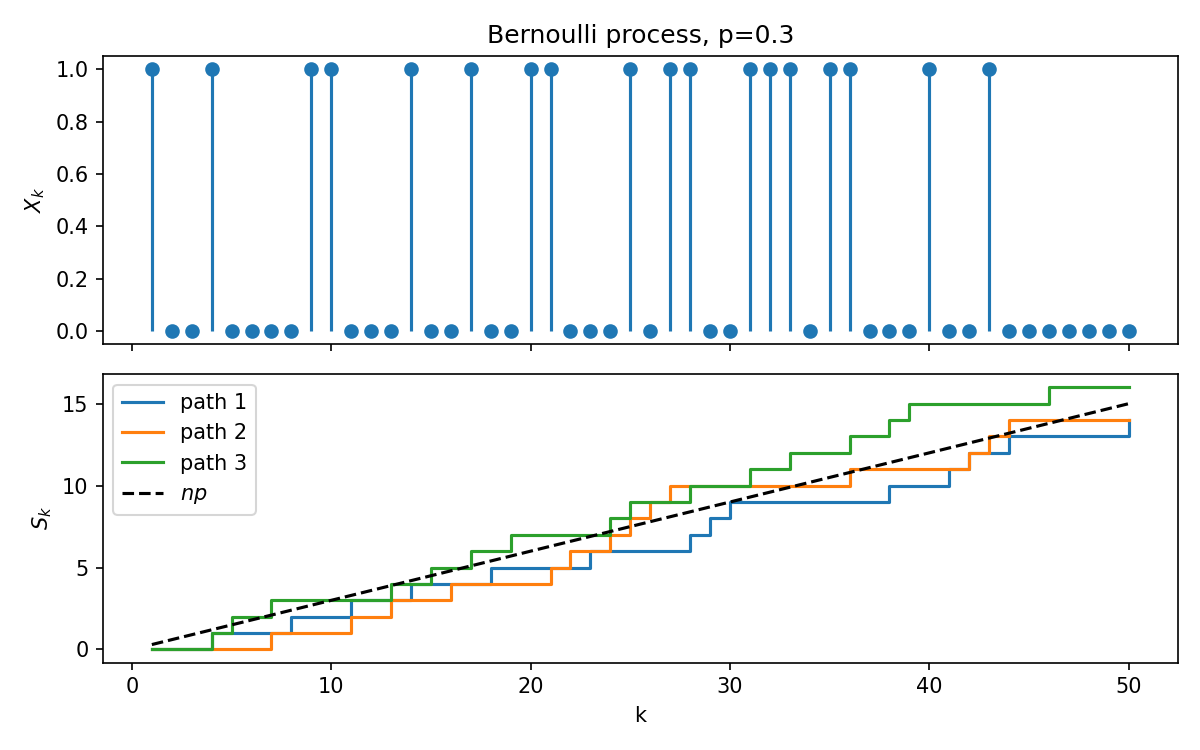
\includegraphics[width=0.85\textwidth]{sample_paths.png}
\caption{Trên: đường mẫu $X_k$ ($p=0{,}3$, $n=50$). Dưới: ba đường mẫu của quá trình đếm $S_k$ và đường kỳ vọng
$np$.}
\label{fig:paths}
\end{figure}

\textbf{Nhận xét (Hình~\ref{fig:paths}).} Các thành công xuất hiện không đều: có những cụm liên tiếp (bước 31--33)
và những đoạn trống dài (bước 44--50), hoàn toàn phù hợp với thời gian chờ hình học có đuôi dài. Các đường $S_k$
dao động quanh đường thẳng $np$ với độ lệch cỡ $\sqrt{npq}$, đúng như~\eqref{eq:binom-moments}.

\subsection{So sánh lý thuyết và mô phỏng}
\begin{table}[ht]
\centering
\caption{So sánh giá trị lý thuyết và mô phỏng ($p = 0{,}3$).}
\label{tab:results}
\renewcommand{\arraystretch}{1.2}
\begin{tabular}{lrrrr}
\toprule
\textbf{Đại lượng} & \textbf{Số lần chạy} & \textbf{Lý thuyết} & \textbf{Mô phỏng} & \textbf{Sai lệch} \\
\midrule
$\E[S_{20}]$ & 20\,000 & 6,000 & 5,982 & $-0{,}3\%$ \\
$\Var(S_{20})$ & 20\,000 & 4,200 & 4,191 & $-0{,}2\%$ \\
$\E[T_1]$ & 20\,000 & 3,333 & 3,343 & $+0{,}3\%$ \\
$\Var(T_1)$ & 20\,000 & 7,778 & 7,715 & $-0{,}8\%$ \\
$\E[T]$ (thí nghiệm không nhớ) & 40\,000 & 3,333 & 3,322 & $-0{,}3\%$ \\
$\E[T-5\mid T>5]$ & 40\,000 & 3,333 & 3,310 & $-0{,}7\%$ \\
\bottomrule
\end{tabular}
\end{table}

Bảng~\ref{tab:results} cho thấy mọi sai lệch đều dưới 1\%, nằm trong mức dao động ngẫu nhiên của trung bình mẫu
với 20\,000--40\,000 lần chạy. Hai dòng cuối kiểm chứng tính không nhớ~\eqref{eq:memoryless}: với điều kiện đã
chờ quá 5 bước, thời gian chờ \emph{thêm} vẫn có trung bình xấp xỉ $1/p \approx 3{,}333$, bằng thời gian chờ ban
đầu.

\begin{figure}[ht]
\centering
\begin{minipage}{0.48\textwidth}
  \centering
  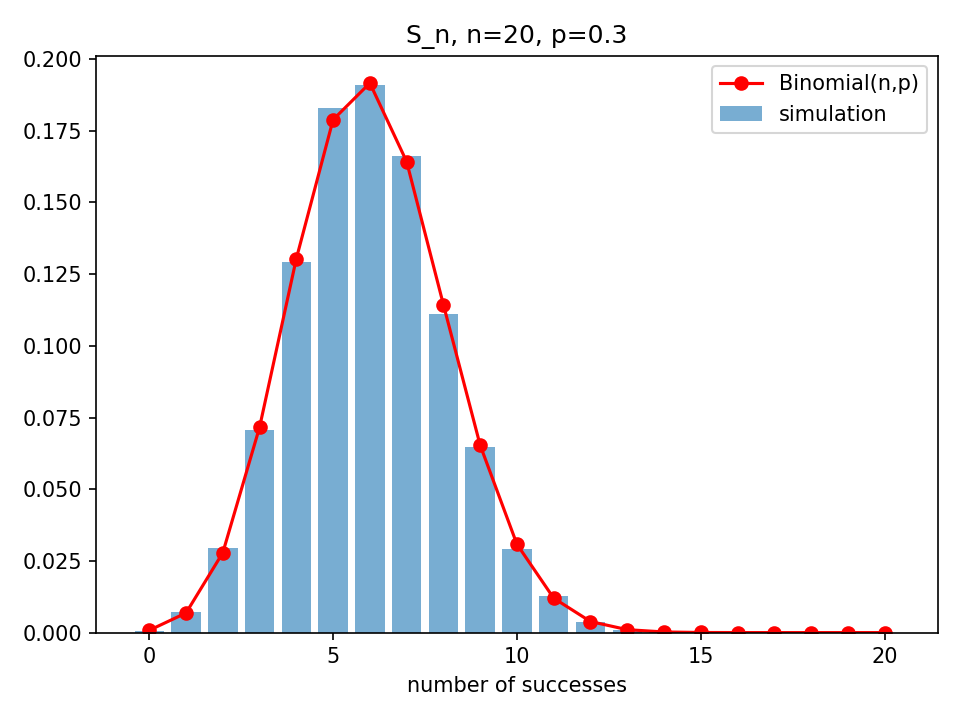
\includegraphics[width=\textwidth]{binomial.png}
  \caption{Phân phối của $S_{20}$: histogram mô phỏng (cột) và pmf nhị thức~\eqref{eq:binom-pmf} (đỏ).}
  \label{fig:binom}
\end{minipage}\hfill
\begin{minipage}{0.48\textwidth}
  \centering
  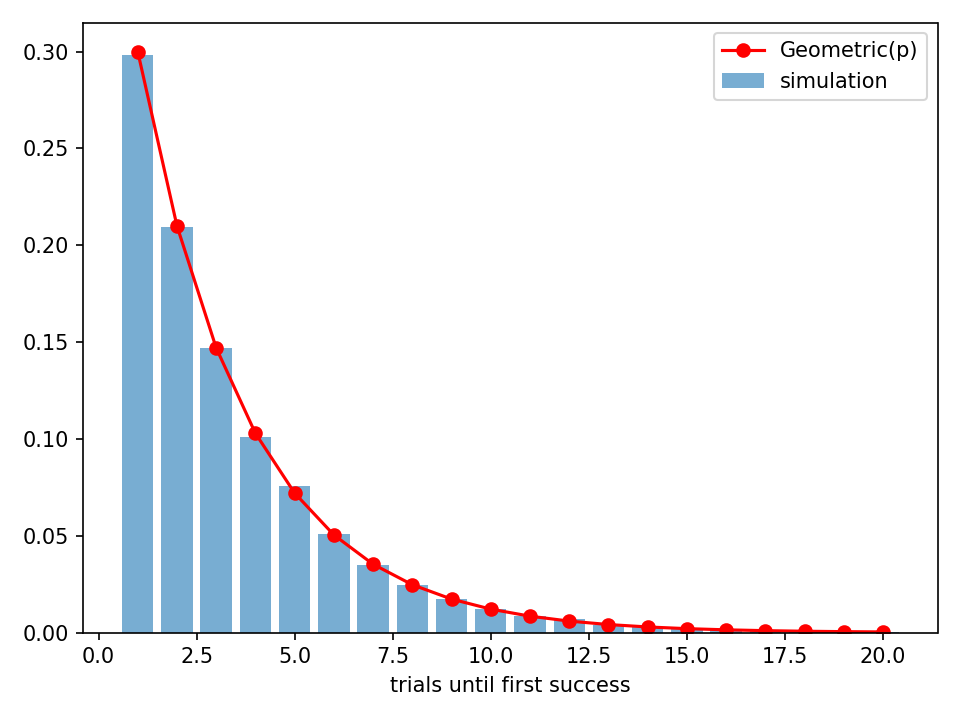
\includegraphics[width=\textwidth]{geometric.png}
  \caption{Phân phối của $T_1$: histogram mô phỏng (cột) và pmf hình học~\eqref{eq:geo} (đỏ).}
  \label{fig:geo}
\end{minipage}
\end{figure}

\textbf{Nhận xét (Hình~\ref{fig:binom} và~\ref{fig:geo}).} Histogram của $S_{20}$ có đỉnh tại 6 (bằng $np$) và
trùng khít với pmf nhị thức. Histogram của $T_1$ giảm theo cấp số nhân với công bội $q = 0{,}7$, đúng dạng
$q^{k-1}p$; cột tại $k=1$ xấp xỉ $p = 0{,}3$.

\begin{figure}[ht]
\centering
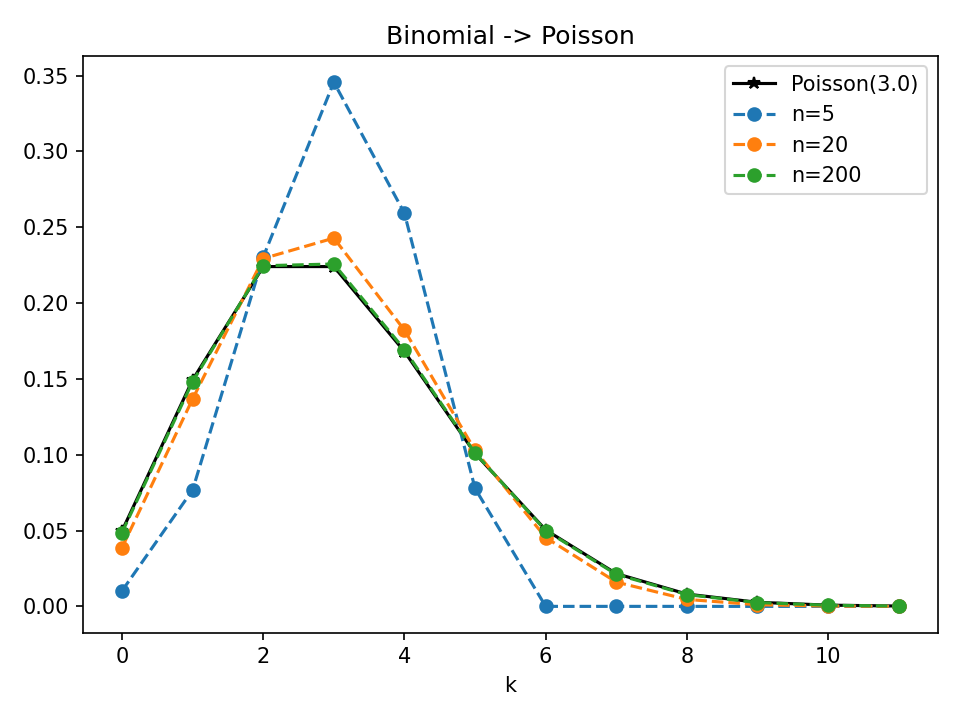
\includegraphics[width=0.6\textwidth]{poisson_limit.png}
\caption{Hội tụ của $\Bin(n, 3/n)$ về $\Pois(3)$ với $n = 5, 20, 200$.}
\label{fig:poisson}
\end{figure}

\textbf{Nhận xét (Hình~\ref{fig:poisson}).} Với $n = 5$ ($p = 0{,}6$) phân phối nhị thức còn khác xa Poisson
(đỉnh nhọn tại 3, bằng 0 từ $k = 6$); với $n = 20$ đã gần; với $n = 200$ hai đường gần như trùng khít, minh hoạ
Mệnh đề~\ref{prop:poisson}.

\FloatBarrier
% =====================================================================
\section{Kết luận}\label{sec:conclusion}
\begin{itemize}
  \item Quá trình Bernoulli là dãy i.i.d.\ $\Bern(p)$ – mô hình đơn giản nhất cho các sự kiện có/không theo thời
        gian rời rạc, xác định hoàn toàn bởi tham số $p$.
  \item Từ nó suy ra phân phối nhị thức (đếm), phân phối hình học và nhị thức âm (chờ), và phân phối Poisson
        (giới hạn). Quá trình có tính không nhớ, gia số độc lập và dừng, và đóng với phép tách/ghép.
  \item Quá trình Bernoulli là phiên bản rời rạc của quá trình Poisson, là trường hợp riêng của xích Markov và là
        nền tảng của bước ngẫu nhiên.
  \item Ba ứng dụng (kiểm soát chất lượng, mạng máy tính, thử nghiệm A/B) cho thấy mô hình trả lời được các câu
        hỏi thực tế, với điều kiện giả thiết độc lập và $p$ không đổi được kiểm tra cẩn thận.
  \item Cài đặt tự viết chỉ dùng \texttt{random.random()} cho kết quả mô phỏng khớp lý thuyết, sai lệch dưới 1\%.
\end{itemize}

% =====================================================================
\FloatBarrier
\begin{thebibliography}{9}
\bibitem{bertsekas}
D.~P. Bertsekas and J.~N. Tsitsiklis, \emph{Introduction to Probability}, 2nd ed., Athena Scientific, 2008,
Chapter~6: The Bernoulli and Poisson Processes. \checkme{số chương/trang theo bản nhóm sử dụng}
\bibitem{ross}
S.~M. Ross, \emph{Introduction to Probability Models}, 12th ed., Academic Press, 2019.
\checkme{chương/mục trích dẫn}
\bibitem{grimmett}
G.~Grimmett and D.~Stirzaker, \emph{Probability and Random Processes}, 4th ed., Oxford University Press, 2020.
\checkme{chương/mục trích dẫn}
\bibitem{crr1979}
J.~C. Cox, S.~A. Ross and M.~Rubinstein, ``Option pricing: A simplified approach,'' \emph{Journal of Financial
Economics}, vol.~7, no.~3, pp.~229--263, 1979.
\end{thebibliography}

% =====================================================================
\appendix
\section{Mã nguồn}\label{app:code}
\IfFileExists{code/bernoulli_process.py}{%
  \lstinputlisting[caption={\texttt{bernoulli\_process.py}},label={lst:full}]{code/bernoulli_process.py}%
}{%
  \lstinputlisting[caption={\texttt{bernoulli\_process.py}},label={lst:full}]{../code/bernoulli_process.py}%
}

\end{document}
